\documentclass[a4paper]{arrowhead}

\usepackage[utf8]{inputenc}
\usepackage[yyyymmdd]{datetime}
\renewcommand{\dateseparator}{-}

\graphicspath{ {fig/} }

\usepackage{adjustbox}


\begin{document}
%% Arrowhead Document Properties
\ArrowheadTitle{Orchestrator System Description}
\ArrowheadType{PUBLIC}
\ArrowheadVersion{G3.2 M2}
\ArrowheadDate{\today}
\ArrowheadAuthor{Csaba Hegedus}
\ArrowheadStatus{Draft}
\ArrowheadContact{hegeduscs@aitia.ai}
\ArrowheadFooter{www.arrowhead.eu}
%%

%% Front Page
\begin{center}
	\vspace*{1cm}
	\LARGE{\arrowtitle}
	\vspace*{1cm}
	
	% Front Page Image
	%\includegraphics{fig/my_image}
	
	\vspace*{1cm}
	\vspace*{\fill}
	
	% Front Page Abstract
	%\begin{abstract}
	%  This is an abstract.
	%\end{abstract}
	
	\vspace*{2cm}
	
	\scriptsize
	\begin{tabularx}{\textwidth}{l X}
		\raisebox{-0.5\height}{\includegraphics[width=2cm]{fig/artemis_logo}} & {ARTEMIS Innovation Pilot Project: Arrowhead\newline
			THEME [SP1-JTI-ARTEMIS-2012-AIPP4 SP1-JTI-ARTEMIS-2012-AIPP6]\newline
			[Production and Energy System Automation Intelligent-Built environment and urban infrastructure for sustainable and friendly cities]}
	\end{tabularx}
	\vspace*{-0.9cm}
\end{center}
\newpage


\section{System Description and Overview}

The Orchestrator provides runtime (late) binding between Application Systems. 

The primary purpose for the Orchestrator System is to provide Application Systems with orchestration information: where they need to connect to. The outcome of the "\emph{Orchestration Service}" include rules that will tell the Application System what Service provider System(s) it should connect to and how (acting as a Service Consumer). Such orchestration rules include:
\begin{itemize}
	\item Accessibility information details of a Service provider (e.g network address and port),
	\item Details of the Service instance within the provider System (e.g. base URL, IDD specification and other metadata),
	\item Authorization-related information (e.g. access token and signature),
	\item Additional information that is necessary for establishing connection.
\end{itemize}

This orchestration rule information can reach the given Application System (consumer) in two different ways: the System itself can request it ("pull") or the Orchestrator itself can update the System when it is needed ("push method"). However, in both cases, there shall be an underlying, hidden process (\emph{"orchestration process"}), which ensures the consistence of state between the various Core Systems.

In G3.2, only the pull method is supported and the Orchestrator shall negotiate with the other Core Systems while trying to facilitate the new service request (or trying to push a new status). This is necessary for the following cases and requirements (basically, when ad hoc, unsupervised connections are not allowed):
\begin{itemize}
	\item When accountability is required for all Systems in the Local Cloud: connections cannot be established without the knowledge, approval and logged orchestration events of the Core Systems ("central governance"). 
	\item QoS and resource management reasons: ad hoc peer-to-peer connections cannot be allowed in certain managed networks and deployment scenarios. Every connection attempt shall be properly authorized and its QoS expectations (resource reservations) handled.  
	\item Inter-Cloud orchestration can only happen via negotiations between the two Core System sets. Ad hoc inter-cloud connections shall not be allowed in the Arrowhead framework. 
\end{itemize}

In these cases, when the Orchestrator is the sole entry point to establishing new connections within the Local Cloud, Application Systems do not have the possibility to skip any of the control loops with all the appropriate Core Systems. When such security and safety concerns are not present, the orchestration process might be cut back or these interactions between Core Systems might be limited. Within G3.2, this is not the primary use case, but it is allowed. With the proper self-implemented (modified) and a self-compiled Orchestrator can fit the deployment best.

 
Therefore, the Orchestrator provides two core Services and may consume many other ones, but at least two -- again, depending on its deployment. Figure~\ref{fig:OrchSys} depicts the mandatory and optional interfaces of this System. 

\begin{figure}[h!]
	\centering
	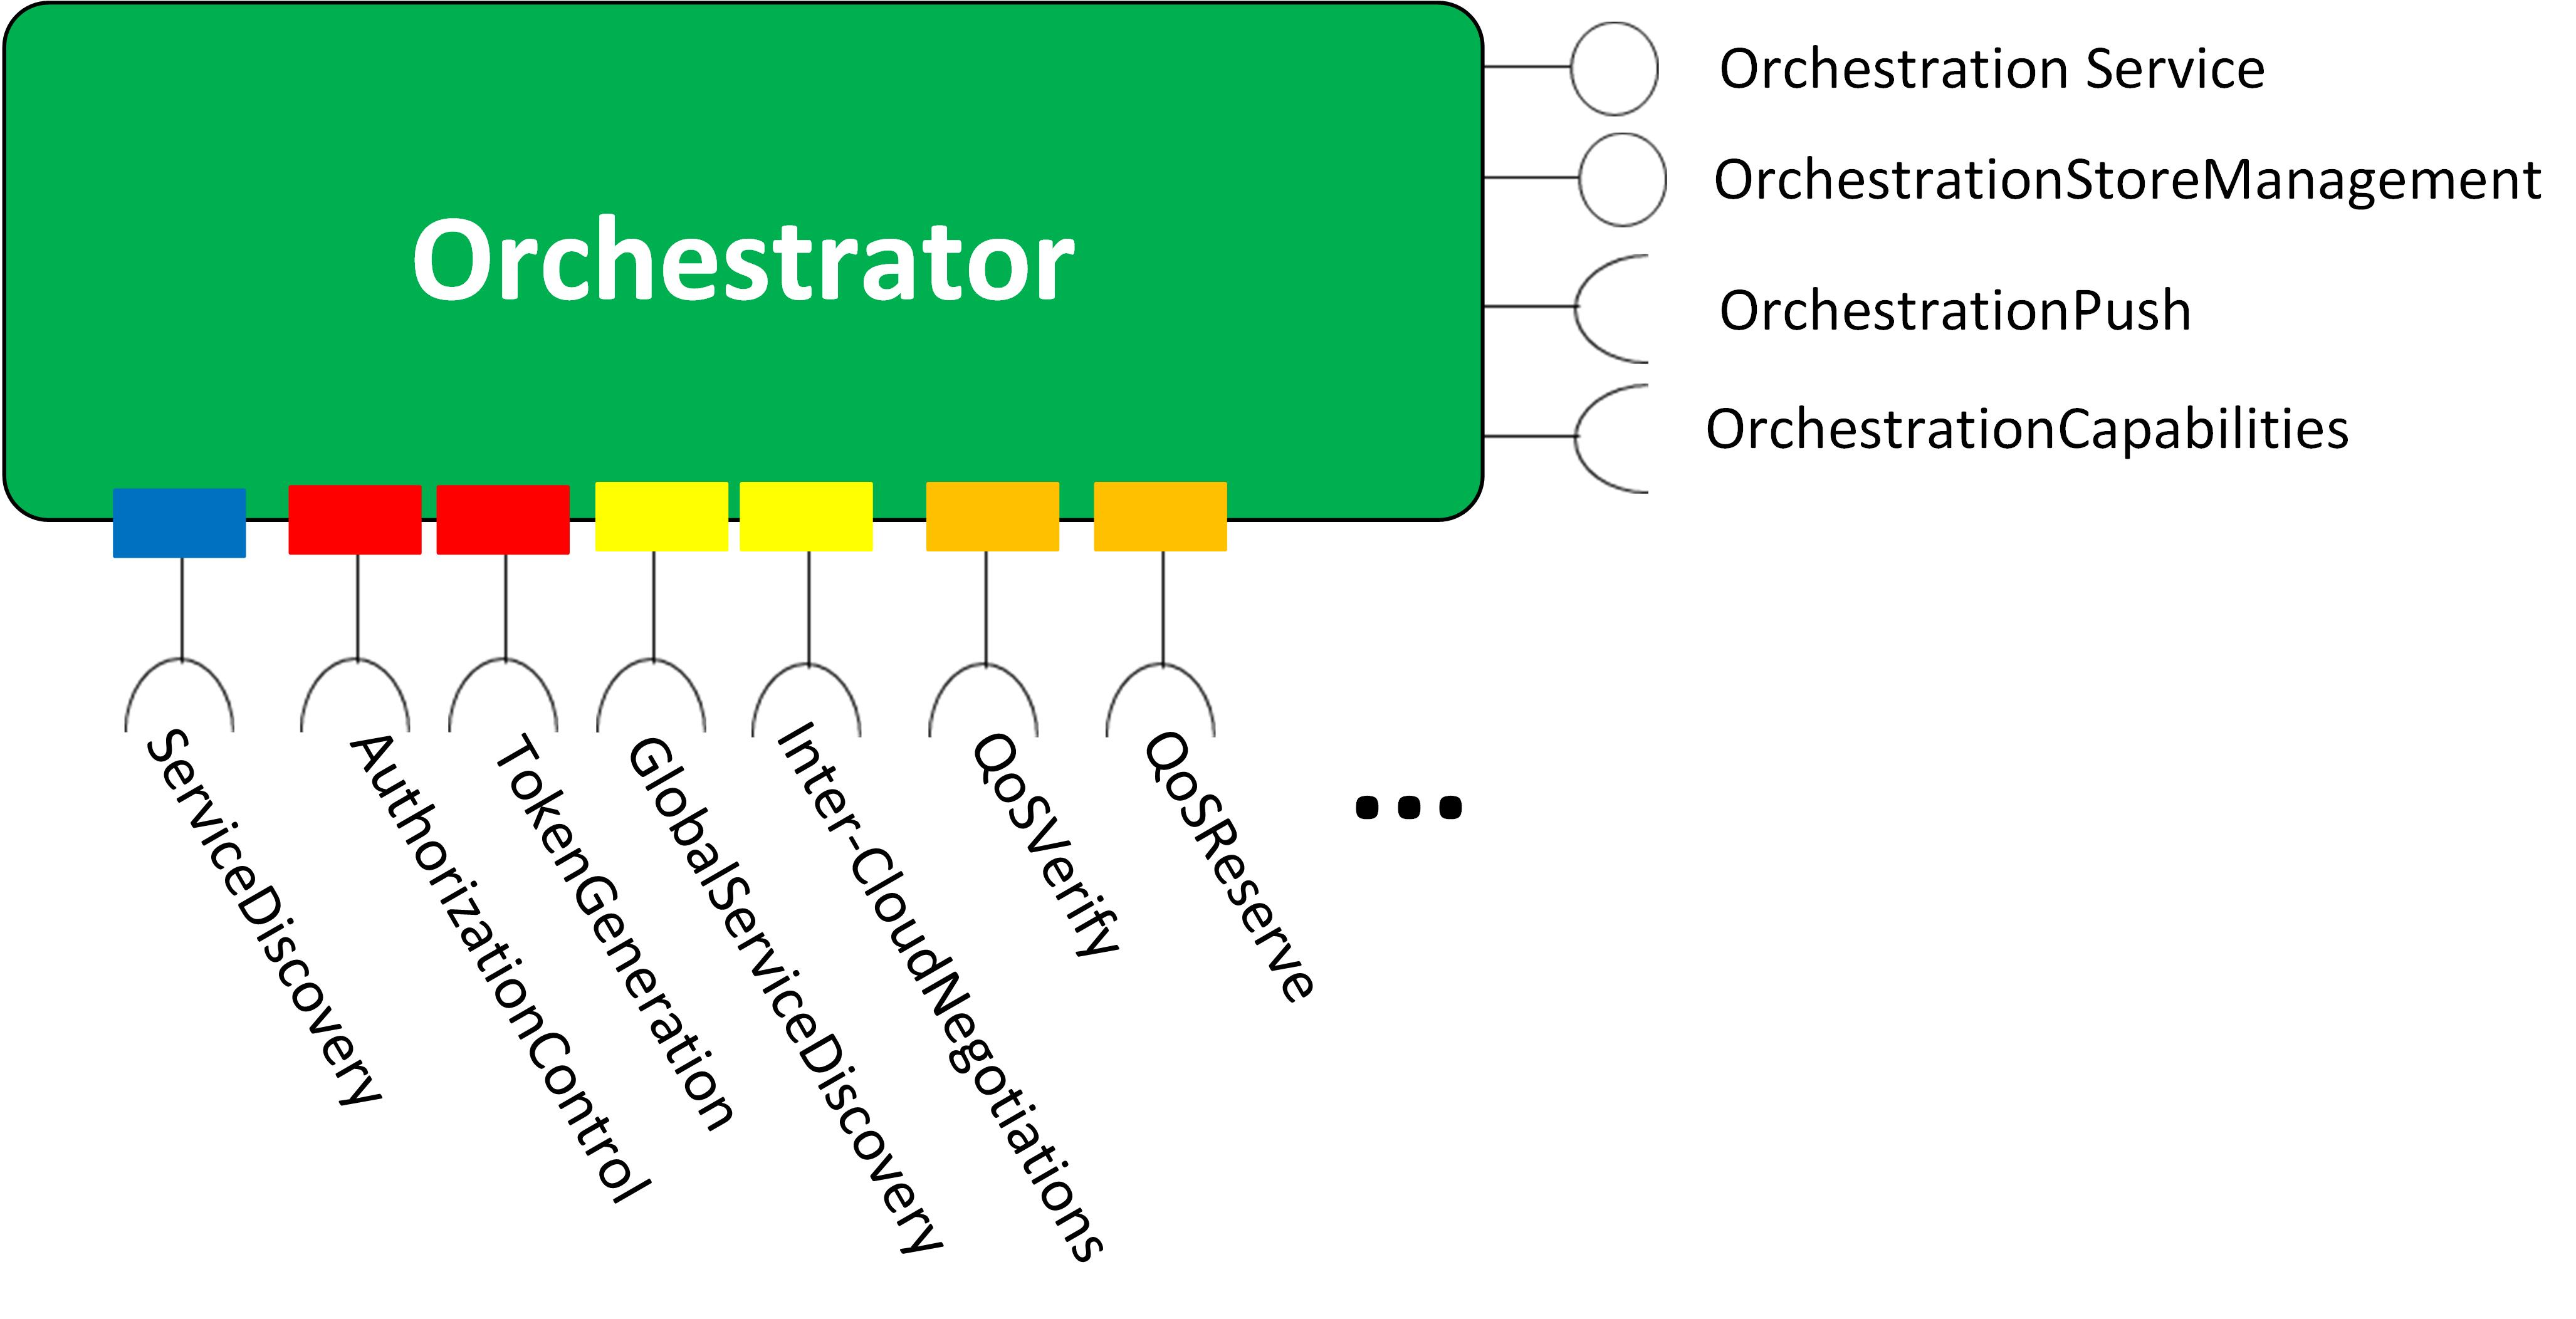
\includegraphics[width=10cm]{fig/orch-sys.jpg}
	\caption{Overview on the Orchestrator System}
	\label{fig:OrchSys}
\end{figure}

In here, the provided Services are:
\begin{enumerate}
	\item Orchestration Service
	\item OrchestrationStoreManagement Service (primarily used by HMI and Plant Description Engine)
\end{enumerate}

Note: G3.2 Milestone 2 currently doesn't implement the Management Service, it will be release in the Milestone 3 version. As a temporary solution, manual modifications in the MySQL database is advised. 


Meanwhile the consumed Services can vary, depending on the instantiation/installation of this System. For example, the Orchestrator can utilize the services of: 
\begin{enumerate}
	\item ServiceDiscovery Service from the ServiceRegistry,
	\item AuthorizationControl Service from the Authorization System,
	\item TokenGeneration Service from the Authorization System,
	\item GlobalServiceDiscovery from the Gatekeeper,
	\item Inter-CloudNegotiations from the Gatekeeper,
	\item QoSVerify from the QoS Manager,
	\item QoSReserve from the QoS Manager,
	\item Logging services from other supporting Systems, e.g. Historian,
	\item and any other service from core systems that are necessary to settle during orchestration.  
\end{enumerate}

The Orchestrator mainly consumes services from other Core Systems in order to fulfill its primary functionality: provide connection targets for Application Systems in a secure and resource managed manner -- hence build an SoS. 

During this \emph{orchestration process} the Orchestrator either facilitates a service request from an Application System or processes a system-of-systems (SoS) level choreography push from the Plant Description Engine ("Choreographer"). For the latter case, the Orchestrator System consumes the OrchestrationPush from affected Application Systems in order to deliver a renewed set of connection rules to them. 

Within the Orchestrator, there is a database which captures design time bindings between Application Systems, the \emph{Orchestration Store}. Operators of the Cloud and other System-of-Systems designer tools ("SoS Choreographers") are allowed to modify the rules stored in the Orchestration Store, other generic Application Systems are not.

The ServiceDiscovery Service is used to publish the Orchestration Service in the Service Registry. This Service is also used to query the Service Registry and fetch (metadata) information on other Application Systems.

The Services of the Authorization System can be used to verify access control and implement other security-related administration tasks. 

The Services of the Gatekeeper can be utilized when inter-Cloud collaboration, servicing is required. 

The Services of the QoS management System can be used to manage device, network and service-level Quality of Service agreements and configurations. 


\section{Use-cases }
For the Orchestrator System, the primary scenario is to provide Application Systems with orchestration information upon request ("\emph{service request}"). The outcome ("\emph{orchestration response}") include orchestration rules that will tell the Application System what service provider(s) it should connect to and how.

An alternative, secondary version of this scenario involves the same information, however, provided by a connection initialized by the Orchestrator, rather than the Application Service itself ("orchestration push"). This is used to relay changes made in the Orchestration Store to the Application Systems ("changes information exchange setup within the SoS"). 

Another scenario is when the Orchestration Store (that stores design time orchestration-related information) of the Orchestrator is being configured via an HMI or via the Plant Description Engine (SoS Choreographer) by the operators of the Local Cloud. 

\newpage
\begin{table}[h]
	\caption{Use case 1}
	\label{table:1}
	\centering
	\begin{adjustbox}{max width=\textwidth}
		\begin{tabular}{|l|l|}
			\hline
			Service Request From Application System &                                                                                                                                                                                                                                                                                  \\ \hline
			ID:                                     & ORCH-PULL                                                                                                                                                                                                                                                                        \\ \hline
			Brief description:                      & An Application System requests a Service.                                                                                                                                                                                                                                        \\ \hline
			Primary actors:                         & Service Consumer System                                                                                                                                                                                                                                                          \\ \hline
			Secondary actors:                       & \begin{tabular}[c]{@{}l@{}}- the other Core System instances of the Local Cloud\\ \\ - the Core Systems instance of another Local Cloud (in case of inter-Cloud orchestration)\end{tabular}                                                                                      \\ \hline
			Preconditions:                          & -                                                                                                                                                                                                                                                                                \\ \hline
			Main flow:                              & \begin{tabular}[c]{@{}l@{}}1- The Application System requests orchestration.\\ \\ 2- The Orchestrator System begins the orchestration process with the other Core Systems.\\ \\ 3- The Orchestrator System responds to the Application System based on the request.\end{tabular} \\ \hline
			Postconditions:                         & -                                                                                                                                                                                                                                                                                 \\ \hline
		\end{tabular}
\end{adjustbox}   
\end{table}

\vspace{5mm}
 
\begin{table}[h]
	\caption{Use case 2}
	\label{table:2}
	\centering
	\begin{adjustbox}{max width=\textwidth}
	\begin{tabular}{|l|l|}
		\hline
		Orchestration information pushed to Application System &                                                                                                                                                                                                                                                                                                                                              \\ \hline
		ID:                                                    & ORCH-PUSH                                                                                                                                                                                                                                                                                                                                    \\ \hline
		Brief description:                                     & The Orchestrator pushes new information on Application Systems.                                                                                                                                                                                                                                                                              \\ \hline
		Primary actors:                                        & Orchestrator                                                                                                                                                                                                                                                                                                                                 \\ \hline
		Secondary actors:                                      & the other Core Systems instances of the Local Cloud                                                                                                                                                                                                                                                                                          \\ \hline
		Preconditions:                                         & There was a change made in the Orchestration Store.                                                                                                                                                                                                                                                                                          \\ \hline
		Main flow:                                             & \begin{tabular}[c]{@{}l@{}}1- The Orchestrator detects a change in the Orchestration Store.,\\ \\ 2- The Orchestrator begins the orchestration process with the other Core Systems for every change in the Store.\\ \\ 3- The orchestrator pushes new connection rules to the Application Systems based on the new Store entry.\end{tabular} \\ \hline
		Postconditions:                                        & -                                                                                                                                                                                                                                                                                                                                            \\ \hline
	\end{tabular}
\end{adjustbox}
\end{table}

\vspace{10mm}

\begin{table}[h]
	\centering
	\caption{Use case 3}
	\label{table:3}
	\begin{adjustbox}{max width=\textwidth}
	\begin{tabular}{|l|l|}
		\hline
		Orchestration information pushed to Application System &                                                                                                                                                                                                                                                                                                                                              \\ \hline
		ID:                                                    & ORCH-PUSH                                                                                                                                                                                                                                                                                                                                    \\ \hline
		Brief description:                                     & The Orchestrator pushes new information on Application Systems.                                                                                                                                                                                                                                                                              \\ \hline
		Primary actors:                                        & Orchestrator                                                                                                                                                                                                                                                                                                                                 \\ \hline
		Secondary actors:                                      & the other Core Systems instances of the Local Cloud                                                                                                                                                                                                                                                                                          \\ \hline
		Preconditions:                                         & There was a change made in the Orchestration Store.                                                                                                                                                                                                                                                                                          \\ \hline
		Main flow:                                             & \begin{tabular}[c]{@{}l@{}}1- The Orchestrator detects a change in the Orchestration Store.,\\ \\ 2- The Orchestrator begins the orchestration process with the other Core Systems for every change in the Store.\\ \\ 3- The orchestrator pushes new connection rules to the Application Systems based on the new Store entry.\end{tabular} \\ \hline
		Postconditions:                                        & -                                                                                                                                                                                                                                                                                                                                            \\ \hline
	\end{tabular}
\end{adjustbox}
\end{table}
\newpage

\section[Behaviour Diagrams]{Behaviour Diagrams}

The orchestration process consists of negotiations with other Core Systems, as Fig.\ref{fig:OrchProc} and \ref{fig:OrchProc2} depict. To be elaborated. 

\begin{figure}[h!]
	\centering
	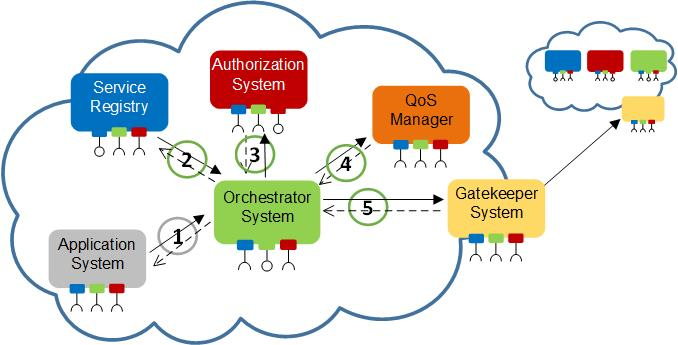
\includegraphics[width=10cm]{fig/orch-proc-v0}
	\caption{Interaction between Core Systems during the orchestration process}
	\label{fig:OrchProc}
\end{figure}

\begin{figure}[h!]
	\centering
	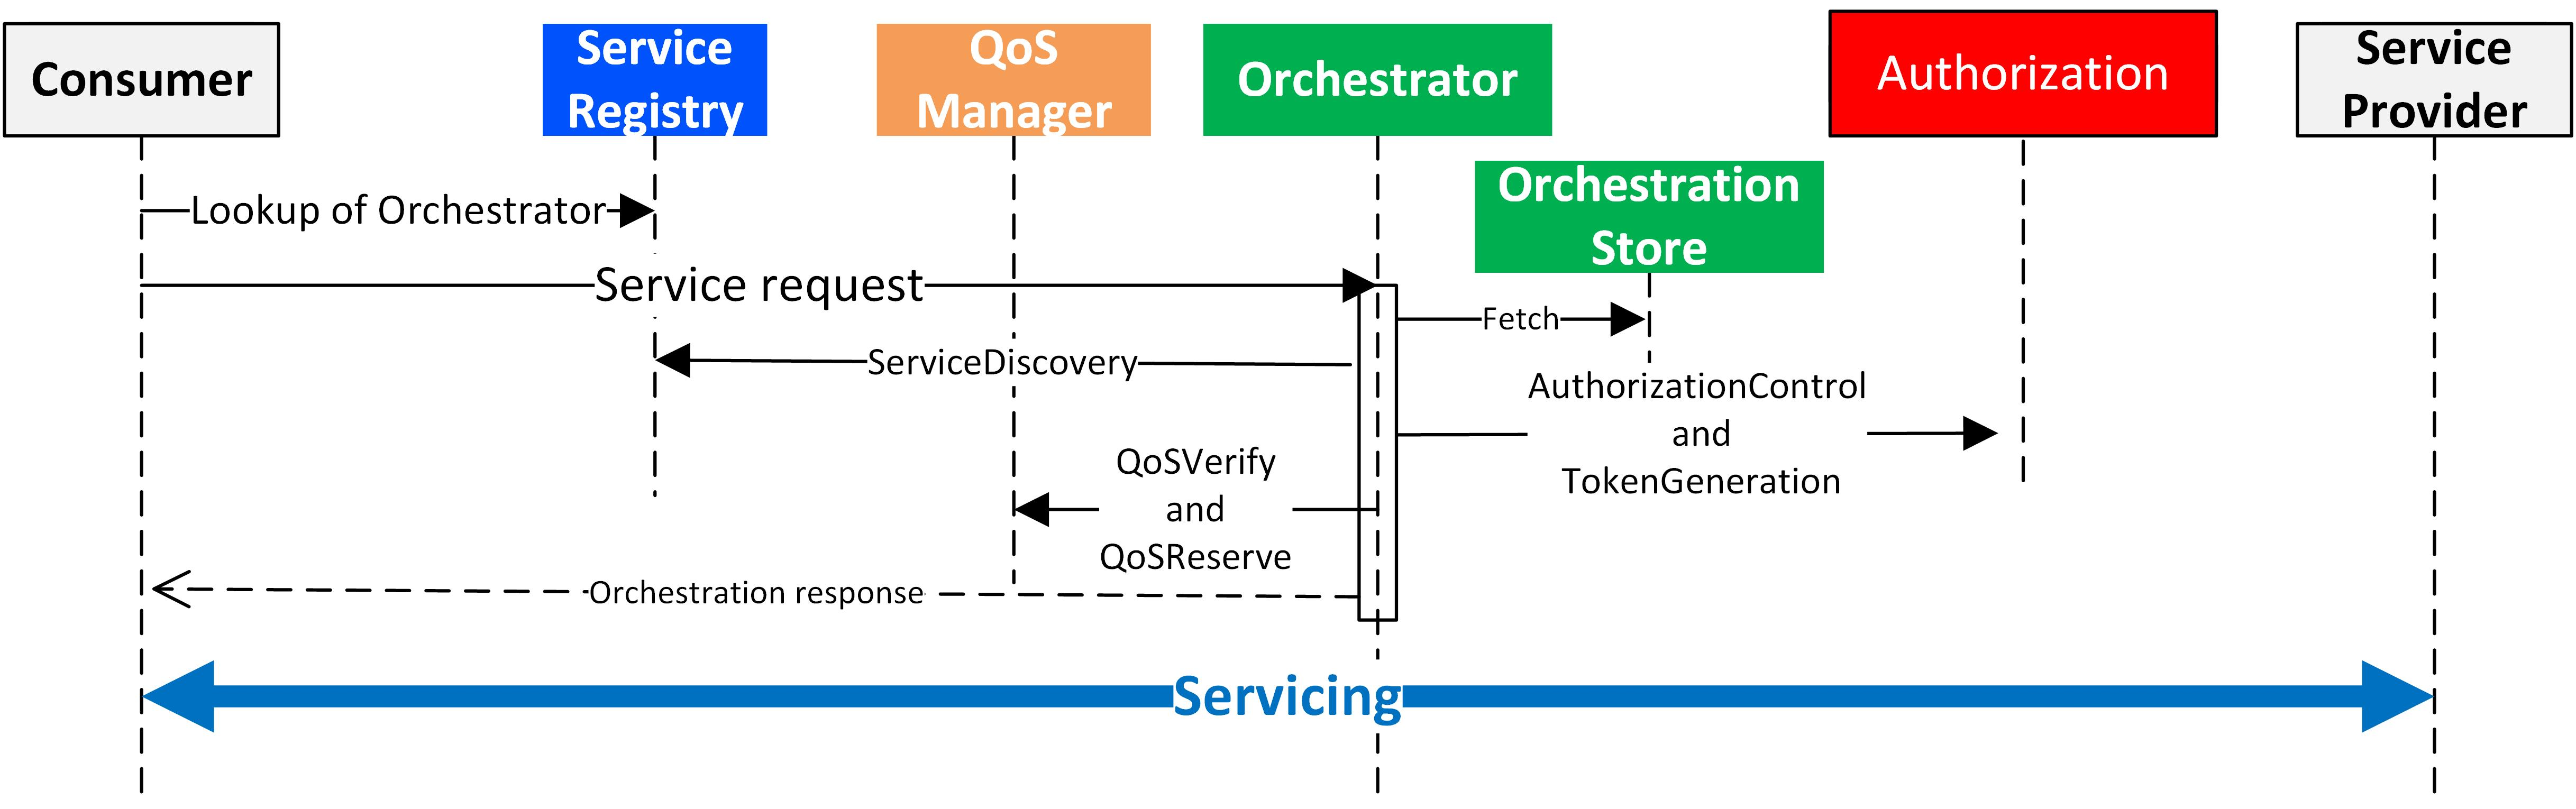
\includegraphics[width=10cm]{fig/intra-orch-proc.jpg}
	\caption{Interaction between Core Systems during the orchestration process}
	\label{fig:OrchProc2}
\end{figure}

\section{Application services}
This section details the Services the Orchestrator provides and might consume.

\subsection[Produced Services]{Produced Services}

\begin{tabular}{|c|c|}
	\hline 
	Service Name & IDD path \\ 
	\hline 
	Orchestration Service & - \\ 
	\hline 
	OrchestrationManagement & - \\ 
	\hline 
\end{tabular} 

\subsection[Consumed Services]{Consumed Services}
Table \stepcounter{Table}{\theTable} Pointers to IDD documents

\begin{tabular}{|c|c|}
	\hline 
	Service Name & Functionality \\ 
	\hline 
	ServiceDiscoveryM2 & Fetch available and suitable Service Providers \\ 
	\hline
	AuthorizationControl & Check access rights \\ 
	\hline 
	TokenGeneration & Generate access tokens \\ 
	\hline
	QoSVerify & Check if the requested QoS level can be met \\ 
	\hline
	QoSReserve & Reserve resource reservations if necessary \\ 
	\hline
	GSD-Init & Discover and look up Service in other Clouds \\ 
	\hline
	ICN-Init& Start negotiations with another Cloud \\ 
	\hline
	
\end{tabular} 

\section{Security }
As a mandatory Core System, the Orchestrator has to be protected at all costs. As this System is a trusted management layer entity -- a decision maker -- within its Local Cloud, its responses are executed by Application Systems. Therefore, the protection of the Orchestrator is of greate essence. In case it is compromised, intruders might be able to reconfigure the general operations of the network. CIAA analysis required for all deployment separately. 

\subsection{Security Objectives}
The Orchestrator's Services have to be available all times.

 The orchestration information provided by this Core System is unique and confidential to its recipient. 
 
 The message from the Orchestrator has to maintain its integrity during transmission. 

\subsection{Assets}
The Orchestration Store poses the only persistent asset of this System. All other assets important in the orchestration process are related to other Core Systems.

\subsection[Non{}-technical Security Requirements]{Non-technical Security Requirements}
 
Scalability of the Orchestrator's Services shall be exampled and set. This issue relates to the maximum practical size of a Local Cloud. 

Error/event handling description is required. How do we detect and then handle when a servicing instance breaks up and requires re-orchestration (e.g. because Service Provider goes offline)? How do we propagate this information towards the QoS Manager and other Core Systems? Clear description of the usage for Event Handler and Historian is required. 

\pagebreak
\section[References]{References}


\section[Revision history]{Revision history}
\subsection[Amendments]{Amendments}

\begin{tabular}{|c|c|c|c|c|}
	\hline 
	No. & Date & Version & Subject of amendments & author \\ 
	\hline 
	1 & 2017. 09. 19. & 0.1 & Initial & Csaba Hegedus \\ 
	\hline 
\end{tabular} 

\subsection[Quality Assurance]{Quality Assurance}
\begin{tabular}{|c|c|c|c|}
	\hline 
	No. & Date & Version & Approved by \\ 
	\hline 
	&  &  &  \\ 
	\hline 
\end{tabular} 
\end{document}
